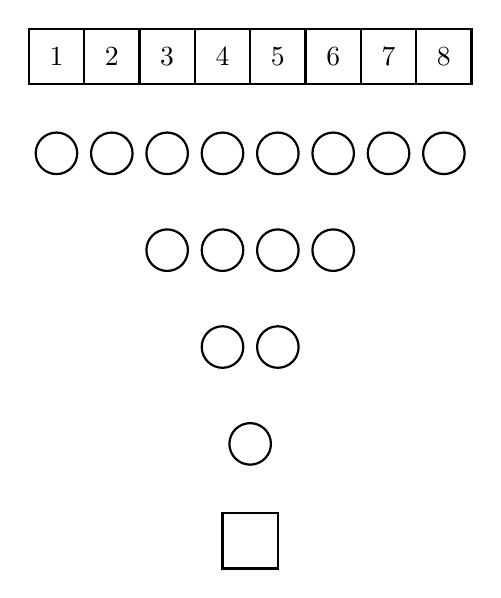
\begin{tikzpicture}

	%% The input row (index = 1)
	\begin{scope}[every node/.style={draw, thick, rectangle, minimum size=2em}]
		%% Iterate from 1-8, storing the index in \n
		\foreach \n in {1,...,8}{%
			\node at (\n*2em, 0) (1-\n) {\n};
		}
	\end{scope}

	%% Iterate through the processing rows
	%% We use a counter to track the row number
	\foreach [count=\r from 2] \m in {8, 4, 2, 1}{%
		%% Calculate the shifts using PGF math
		\pgfmathsetmacro\xShift{(8-\m)/2*2em}
		\pgfmathsetmacro\yShift{(\r-1)*-3.5em}

		\begin{scope}[every node/.style={draw, thick, circle, minimum size=1.5em}, xshift=\xShift, yshift=\yShift]
			\foreach \n in {1,...,\m}{%
				\node at (\n*2em, 0) (\r-\n) {};
			}
		\end{scope}
	}

	%% The output row
	\node at (9em,-17.5em) [draw, rectangle, thick, minimum size=2em] (6-1) {};

\end{tikzpicture}
